\chapter{Analýza}

\begin{chapterabstract}
Tato kapitola analyzuje nástroje a frameworky pro tvorbu a správu výukových materiálů, včetně jejich předností, nedostatků a podpory interaktivity. Zaměřuje se na tradiční i moderní nástroje, otázky komunitního rozšíření a bezpečnosti. V závěru jsou definovány klíčové požadavky na uživatele aplikace a funkčnosti, které je třeba řešit při návrhu platformy.
\end{chapterabstract}


\section{Správa a tvorba materiálů pro výuku}


Do vzdělávacího procesu mimo klasické metody patří tvorba a distribuce výukových materiálů.
Mezi výukové materiály lze zahrnout například prezentace, skripta, plakáty, interaktivní hry, doplňovačky, testy, simulační modely nebo audiovizuální obsah.
V posledních letech, díky rozvoji digitálních technologií, je stále důležitější sdílet materiály online, aby studenti mohli pracovat samostatně nebo v týmech a měli k materiálům přístup kdykoliv.

Online sdílení materiálů umožňuje rychlou aktualizaci obsahu, což je zvláště důležité v případech, kdy se výukový obsah mění nebo vyvíjí v reakci na aktuální potřeby studentů nebo průběh výuky.
Navíc umožňuje učitelům flexibilně přizpůsobovat obsah individuálním potřebám jednotlivých studentů nebo skupin.

Dalším přínosem je možnost zpětné vazby v reálném čase, kdy studenti mohou přímo komentovat, odpovídat a reagovat na obsah materiálu.

Mezi platformy vhodné pro distribuci~\cite{msmt_aplikace} výukových materiálů patří například Microsoft Teams, Bakaláři, Google Disk a Google Classroom, Škola Online nebo další obdobné služby.
Tyto platformy často umožňují integraci s jinými nástroji, jako jsou kalendáře, nástroje pro komunikaci nebo aplikace na zadávání úkolů, což zjednodušuje organizaci výukového procesu.

Každá z těchto platforem má své specifické funkce -- například Microsoft Teams podporuje synchronní i asynchronní komunikaci mezi učiteli a studenty~\cite{teams}, zatímco Google Disk poskytuje možnost snadného sdílení a spolupráce na dokumentech v reálném čase.
V některých případech však tyto nástroje mohou být omezené, například z hlediska podpory různorodých formátů materiálů nebo absence pokročilých funkcí pro práci s interaktivními prvky.

I když se tato práce primárně nezabývá distribucí materiálů, je nezbytné, aby navrhovaná aplikace umožňovala sdílení obsahu pomocí odkazů.

Nástroje pro tvorbu výukových materiálů zahrnují Google Slides, PowerPoint, Microsoft Word, \LaTeX, Canva a mnoho dalších, což podrobněji rozebírám v následujících kapitolách.
Učitelé často využívají širokou škálu nástrojů, protože žádný z existujících nástrojů není zcela dokonalý a není jednoduché vytvořit univerzální řešení.
To způsobuje značnou míru zmatení u studentů a ztěžuje práci učitelům.

\subsection{Vlastní zkušenosti}

Žádná z klasických platforem na sdílení výukových materiálů a hodnocení mi plně nevyhovovala, což mě vedlo k tomu, abych si v rámci své bakalářské práce vytvořil vlastní portál~\cite{cajthaml_bp}.
Tento portál umožňuje nejen sdílení materiálů, ale také zajišťuje automatickou interaktivitu, například tím, že studenti si mohou během hodiny zapisovat poznámky přímo do systému.
Taktéž poskytuje další mnoho věcí, jako flexibilní hodnocení či motivační a gamifikační prvky.

V minulosti jsem používal v podstatě všechny nástroje zmíněné dříve i později, ať už pro tvorbu materiálů, jejich sdílení nebo interaktivní výuku.

Pro prezentace nyní často využívám RevealJS, který však má jistá omezení, jak podrobněji rozebírám v následujících kapitolách.
Skripta vytvářím buď přímo ve svém systému, nebo za pomoci LaTeXu, a pro tvorbu herních a interaktivních aktivit používám nástroje jako Blooket, JeopardyLabs a mnoho dalších služeb.

Rozdělení různých typů materiálů do více platforem mi však nevyhovuje, protože jejich správa je zbytečně složitá a časově náročná.
Právě tato zkušenost vedla k záměru této diplomové práce, jejímž cílem je vytvořit jednotnou platformu, která spojí různé typy materiálů a umožní jejich snadné rozšíření a úpravy.

Ze zpětných vazeb studentů, které pravidelně sbírám na konci školního roku, často zaznívá, že interaktivita materiálů je nedostatečná a že jejich používání je kvůli tomu složité a neintuitivní.
Tato zpětná vazba dále zdůrazňuje potřebu vytvořit systém, který by byl přehledný, interaktivní a přizpůsobitelný jak pro učitele, tak pro studenty.

\subsection{Dotazník}

Prozatím si nejsem jistý, zda je to dobrý nápad.\todo{Provést?}

\section{Aplikace na tvorbu prezentací}

Nejpřirozenějším základem pro výuku je prezentace, která podporuje a vizualizuje myšlenky učitele před skupinou studentů.
Správně strukturovaná prezentace poskytuje kostru výkladu, umožňuje přehledné předání látky a pomáhá udržet pozornost publika.
Na trhu existuje celá řada nástrojů určených pro tvorbu prezentací, lišících se funkcionalitou, mírou interaktivity, možnostmi spolupráce a také obtížností při vytváření obsahu.
Následující podkapitoly popisují vybrané zástupce, které jsou pro mou budoucí práci relevantní.

\subsection{PowerPoint}

PowerPoint, součást balíku Microsoft Office, je dlouhodobě vnímán jako standard~\cite{pp_usage} v oblasti tvorby prezentací.
Mnoho uživatelů jej zná díky intuitivnímu rozhraní a širokému spektru funkcí~\cite{pp_usage}.
Hlavní výhody PowerPointu spočívají v jeho univerzálnosti, snadné obsluze a perfektní provázanosti s dalšími nástroji Microsoft Office, jako jsou Word či Excel~\cite{pp_excel, pp_word}.
Nabízí také velkou knihovnu šablon, grafů, přechodových efektů a základní možnosti vkládání multimédií.

Nevýhodou může být omezená kreativita u některých uživatelů vyplývající z lineárního uspořádání snímků a složitého nebo omezeného používání interaktivních prvků. 
Častým problémem je i kompatibilita mezi staršími a novějšími verzemi formátů.
Přestože PowerPoint existuje i ve webové verzi umožňující spolupráci v reálném čase, tato online varianta je funkcemi oproti desktopové verzi značně omezena~\cite{pp_platforms}.
Další nevýhodou je cena –- přístup k plné verzi aplikace je placený, a to často brzdí její širší využití zejména ve školách s omezenými rozpočty.

\subsection{Google Slides}\label{text:google_slides}

Google Slides je bezplatný webový nástroj pro tvorbu prezentací od společnosti Google. 
Hlavní přednosti spočívají v možnostech snadné spolupráce více uživatelů v reálném čase~\cite{slides}, neboť dokument lze sdílet a společně editovat odkudkoli.
Integrace s ostatními službami Google (Disk, Dokumenty, Tabulky) umožňuje jednoduchý import a export různých typů souborů, a díky tomu se výrazně usnadňuje týmová práce a přístup ke společným materiálům. 
Ve výchozím stavu je služba zdarma, avšak pokročilé funkce a správa dat jsou často vázány na účet v rámci Google Workspace~\cite{slides}, který mohou organizace platit v rámci firemního nebo institucionálního předplatného. 

Výhodou je automatické ukládání na cloud, takže není nutné se obávat ztráty dat~\cite{slides}, a navíc je vše dostupné na více zařízeních, což usnadňuje vzdálený přístup k prezentacím. 
Na druhou stranu je nezbytné mít stabilní připojení k internetu a být obezřetný vůči ukládání citlivých údajů do cloudu, protože Google Slides shromažďuje metadata o aktivitě uživatelů (například informace o tom, kdo a kdy dokument editoval)~\cite{google_terms}, což může s ohledem na soukromí a bezpečnost některým institucím či uživatelům vadit. 
Dále je možné, že prezentace vytvořené v Google Slides nebudou stoprocentně kompatibilní s PowerPointem a jinými nástroji zejména ve svojí interaktivitě a pluginy, což může způsobit problémy při přenosu mezi různými platformami. 
Nevýhodou jsou také omezenější pokročilé funkce, animace či grafické úpravy oproti PowerPointu nebo jiným specializovaným nástrojům. 

Google Slides nicméně celkově nabízí snadno použitelný a přístupný nástroj pro spolupráci a rychlou tvorbu prezentací, který uživatelům postačí pro většinu běžných scénářů, obzvláště tam, kde je důraz na flexibilitu, týmovou práci a okamžitý vzdálený přístup k materiálům.


\subsection{RevealJS}

RevealJS je knihovna a framework, která dovoluje tvořit prezentace pomocí zdrojového kódu v \texttt{HTML}. 
Výsledné prezentace jsou k dispozici jako webová stránka~\cite{revealjs}, ve které se vykreslují jednotlivé snímky, mezi kterými lze plynule procházet. 
Velkou výhodou RevealJS je široká komunita, řada open-source pluginů a neomezené možnosti integrace multimediálního obsahu, od videí přes animace až po spustitelný kód. 
Nevýhodou může být různé zpracování, dokumentace a nastavení pluginů, které nemusí být vždy vzájemně kompatibilní, nutnost znalostí webových technologií a absence \texttt{WYSIWYG} editoru. 

Vytvořené prezentace je často nutné hostovat v cloudu, zejména pokud používají pluginy vyžadující serverové prostředí.
Společnost, která vytvořila RevealJS, taktéž vytvořila službu Slides.com~\cite{revealjs, slidescom}, umožňující tvořit prezentace pomocí editoru s frameworkem RevealJS, s prémiovými pluginy a automatickým cloudovým uložením, avšak tento nástroj je kódově uzavřený a placený. 

Osobně jsem RevealJS knihovnu již řadu let používal pro tvorbu prezentací pro své studenty, kteří ocenili možnost vytvářet v prezentaci interaktivní prvky, jako je například kódový blok s okamžitým zobrazením výsledku. 
Na obrázku \ref{fig:analyza:revealjs-ukazka} je vidět příklad takové prezentace, kde je vlevo kód a vpravo výsledek zobrazený v prohlížeči, což podporuje lepší pochopení učiva a aktivní zapojení studentů. 

Zajímavou funkcí jsou i tzv. vertikální snímky, které umožňují nelineární strukturování prezentace, kdy se lze pohybovat nejen horizontálně, ale i vertikálně v rámci logických celků prezentace.
Celkově si lidi chválí i možnost modularity těchto snímků a že je velmi jednoduché spojovat jednotlivé atomické skupiny do větších celků.


\begin{figure}[h!]
    \centering
    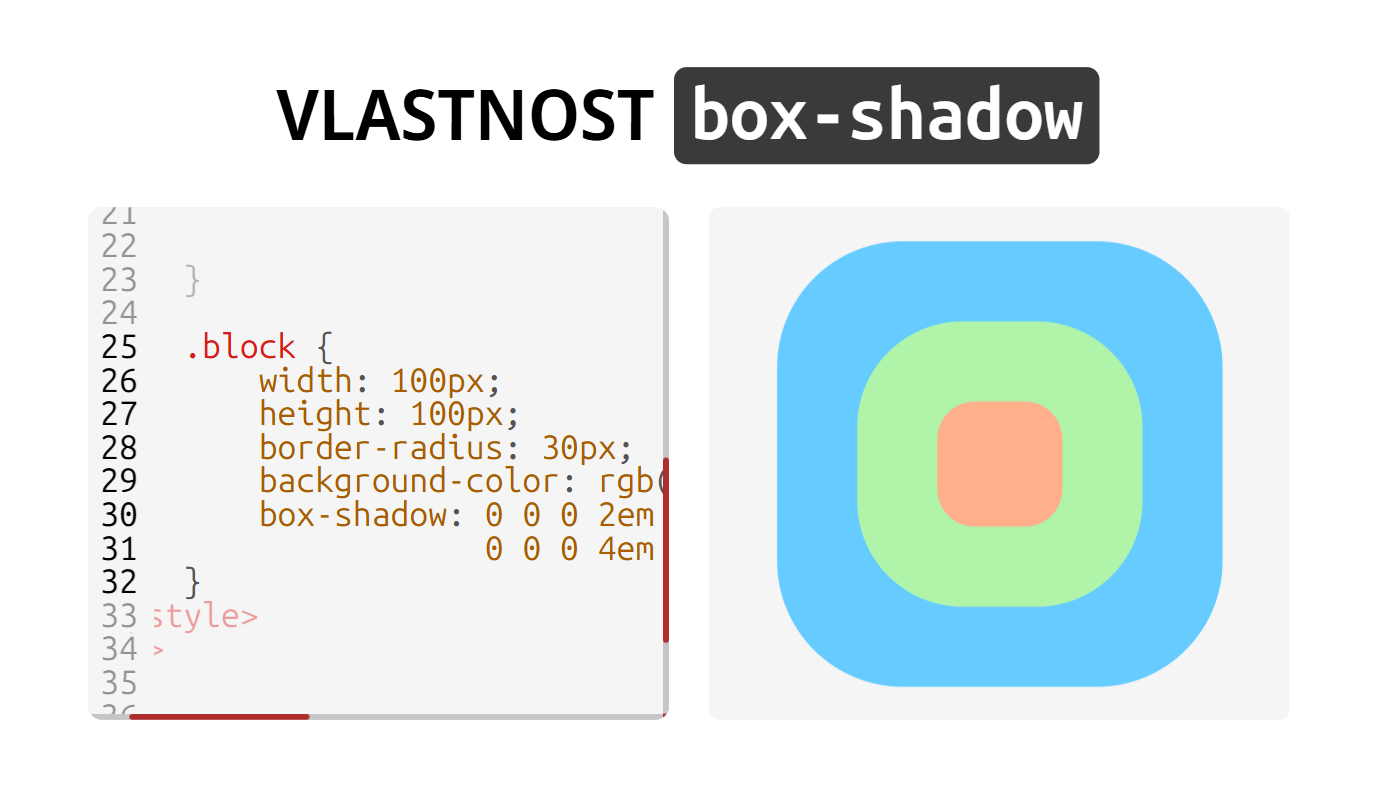
\includegraphics[width=0.9\linewidth]{media/03_analyza/revealjs.png}
    \caption{RevealJS prezentace s rozdělením kódu a výsledku}
    \label{fig:analyza:revealjs-ukazka}
\end{figure}

\subsection{Beamer v \LaTeX}

Beamer je třída v sázecím systému \LaTeX, která se zaměřuje na vytváření snímkových prezentací.
Nejvíce je Beamer společně s \LaTeX~populární v akademickém prostředí zejména z důvodu jednoduchého sázení matematických formulí a zápisu pomocí kódového jazyka, který leccos dovoluje. 

Zápis je ale zároveň to nejvíce nenáviděné na \LaTeX~\cite{latex_reddit}, a to zejména z důvodu kryptických kódových chyb a různých zastaralých zápisů.
Vygenerované prezentace jsou taktéž statické a nedá se v nich dělat jakákoliv interaktivity. 
Výhodou takovéto kódové generace je, že často z jednoho zdrojového kódu -- pro prezentaci -- se dají tvořit taktéž skripta a to tím, že přidáváme takové bloky kódu, které vykreslí právě v jednom nebo v obou módech.

\section{Aplikace na grafickou tvorbu}

Tato sekce se zaměřuje na nástroje, které umožňují snadno a rychle vytvářet vizuálně atraktivní materiály, ať už jde o grafiky, ilustrace, uživatelská rozhraní či jiné kreativní prvky doplňující prezentace a vzdělávací materiály.

\subsection{Canva}\label{text:canva}

Canva je webová platforma pro rychlou a snadnou tvorbu grafických materiálů, jako jsou plakáty, letáky, sociální příspěvky či prezentace, s bohatou nabídkou šablon, fontů a grafických prvků\todo{Zdroj}. 
Hlavní výhody Canvy spočívají v intuitivním uživatelském rozhraní\todo{Zdroj}, obrovské knihovně předpřipravených šablon a prvků, možnosti drag-and-drop úprav a snadné integraci multimédií.

Díky cloudovému prostředí umožňuje Canva týmovou spolupráci\todo{Zdroj}, sdílení souborů v reálném čase a přístup k materiálům odkudkoli, přičemž většina základních funkcí je dostupná zdarma. 

Nevýhodou může být omezenější možnost zcela individuálního designu u některých šablon, menší preciznost u specifických grafických úprav a u pokročilých funkcí potřeba placené verze Canva Pro. 
Přesto je Canva velmi oblíbená pro rychlou tvorbu vizuálně atraktivních materiálů i mezi pedagogy, kteří nepotřebují pokročilé znalosti grafických programů a chtějí rychle připravit poutavé grafické materiály či prezentace.
Čeští pedagogové mají program Canva k dispozici zdarma po ověření\todo{Zdroj}. Tento nástroj je mezi pedagogy velmi oceňován zejména právě pro jeho jednoduchost\todo{Zdroj}.

\subsection{Figma}\label{text:figma_popis}

Figma je profesionální online nástroj pro design a prototypování uživatelských rozhraní, který se v posledních letech stal standardem v oblasti webového a aplikačního designu\todo{Zdroj}. 
Nabízí vektorový grafický editor, možnost vytvářet interaktivní prototypy a sdílet je v reálném čase s kolegy, což výrazně usnadňuje spolupráci v týmech\todo{Zdroj}. 
Velkou předností Figmy je její cloudové prostředí, ve kterém se změny ukládají automaticky, a každý člen týmu vidí okamžité aktualizace, což zjednodušuje proces zpětné vazby a revizí. 

Nevýhodou může být vyšší křivka učení pro uživatele neznalé profesionálních grafických nástrojů a nutnost stabilního připojení k internetu, aby bylo možné plně využít funkce Figmy. 
Přesto Figma představuje výkonný a flexibilní nástroj, který může pedagogům a školám pomoci při tvorbě interaktivních rozhraní pro studijní materiály, e-learningové platformy či jiné digitální vzdělávací projekty.

\section{Aplikace na tvorbu materiálů}\todo{Celkově k tomuhle dopsat spoustu věcí}

Tato sekce představuje nástroje, jež umožňují připravovat a distribuovat výukové materiály v podobě interaktivních prezentací, kvízů, vizuálních map či jiných vzdělávacích formátů.
Tyto nástroje tedy cílí na velmi podobné cíle, které má i moje budoucí aplikace.
Hlavním cílem těchto aplikací je zefektivnit a zpestřit proces učení, zvýšit zapojení studentů a nabídnout pedagogům možnosti, jak obohatit svou výuku o moderní a atraktivní formy obsahu.

\subsection{Genially}

Genially je online platforma pro tvorbu interaktivních materiálů, prezentací, infografik a dalších multimediálních podkladů, které mohou publikum aktivně zapojit do obsahu.
Platforma je navržena s důrazem na jednoduchost použití, aby byla dostupná jak profesionálům, tak i laikům.

Jednou z klíčových vlastností Genially je možnost rychlého přidávání interaktivních prvků\todo{Zdroj}, jako jsou kvízy, hypertextové odkazy, animace a různorodý multimediální obsah. 
Tyto funkce nejen zvyšují zapojení studentů, ale také podněcují jejich motivaci k učení skrze aktivní interakci s obsahem. 
Tím se platforma stává nejen nástrojem pro prezentaci informací, ale také prostředkem pro výuku založenou na principu konstruktivistické pedagogiky\todo{Zdroj}. 
% Konkrétní příklady interaktivních prvků zahrnují již zmíněné odkazy, kliknutí, řazení, kvízy, interaktivní aplikace uvnitř a mnoho dalšího.

Velkou předností Genially je jeho intuitivní rozhraní a široká škála připravených šablon.
Tyto šablony jsou navrženy s ohledem na vizuální atraktivitu a dynamiku, což umožňuje rychlou tvorbu obsahu bez nutnosti pokročilých grafických znalostí.
Platforma tak poskytuje tvůrcům nástroje, které by jinak vyžadovaly komplexní software a odborné znalosti.

Genially je však placená služba, což může představovat značnou překážku pro vzdělávací instituce a jednotlivce s omezenými finančními zdroji. 
Bezplatná verze nabízí pouze omezenou funkcionalitu a materiály vytvořené v rámci této verze obsahují vodoznak.
Dále je export obsahu možný pouze u placených tarifů, a to v různých formátech, jako jsou PDF nebo HTML. 
Tato omezení mohou snižovat flexibilitu uživatele, který by chtěl svůj obsah sdílet, archivovat offline a nebo celkově více plánovat výuku. 
Zároveň nelze provádět vlastní úpravy kódu ani integrovat komunitní rozšíření, což omezující uživatele, kteří by potřebovali pokročilé nebo zcela unikátní funkce.

Je třeba zmínit, že Genially jako firma je formálně napojena na platformu Canva\todo{Zdroj}, viz kapitola \ref{text:canva}, a tyto dvě služby sdílejí základ vizuálního editoru. 
Tento aspekt zvyšuje celkovou kvalitu uživatelského zážitku, protože editor se vyznačuje vysokou přehledností a snadnou manipulací s obsahem. 
Z tohoto pohledu lze považovat Genially za nástroj, který efektivně staví na osvědčených principech uživatelského designu a zajišťuje širokou dostupnost profesionálních vizuálních standardů.

Na základě vlastních zkušeností jsem využil Genially pro tvorbu několika prezentací a vzdělávacích materiálů. 
Zatímco samotná tvorba byla rychlá a relativně bezproblémová, setkala jsem se s určitými nedostatky, které ztěžovaly optimální využití platformy. 
Jedná se o:\todo{Dopsat}

\begin{itemize}
    \item omezenost obsahu
    \item limitace "klávesnice"
\end{itemize}

NÁZOR OSTATNÍCH\todo{najít}

\subsection{Mentimeter}

Mentimeter je webová aplikace určená pro interaktivní zapojení publika prostřednictvím online hlasování, dotazníků, kvízů, slovních mraků, průzkumů a anket\todo{Zdroj}. 
Umožňuje učitelům a přednášejícím získávat okamžitou zpětnou vazbu od studentů, což napomáhá identifikovat oblasti nepochopení, zvýšit míru interakce a podporovat aktivní účast na výuce. 

Velkou předností Mentimeteru je jeho uživatelská přívětivost, široká nabídka interaktivních formátů, kompatibilita s mobilními zařízeními a snadná integrace do výukových scénářů, přičemž výsledky lze ihned zobrazit na obrazovce. 
Vzhledem k tomu, že Mentimeter se zaměřuje zejména na interakci a aktivní zapojení publika, nikoliv na obsah samotný, nenabízí mnoho grafických funkcí pro tvorbu složitých nebo vizuálně bohatých materiálů\todo{Zdroj}. 

Stejně jako Genially zde chybí komunitně tvořené rozšíření a detailní možnosti kódových úprav, avšak pokud je cílem zvýšit interaktivitu a okamžitou odezvu od studentů, Mentimeter tento úkol splní velmi dobře.

Mentimeter jsem aplikoval několikrát ve výuce a splnil to, co jsem očekával, a to, že se zvýšila interaktivita ve výukové skupině. 
Velkým problémem je opravdu to, že obsah nejde upravovat natolik, aby šlo vytvořit cokoliv. 
V aplikaci taktéž velmi chybí grafické možnosti, na jednotlivé snímky lze vložit pouze jeden interaktivní prvek s jednotkami grafických variací.

NÁZOR OSTATNÍCH\todo{najít}

\subsection{Prezi}

Prezi je prezentační nástroj, který se odlišuje od klasických lineárních prezentací svou nelineární strukturou.
Místo jednotlivých snímků pracuje Prezi s jedním velkým plátnem\todo{Zdroj}, na němž lze rozmístit text, obrázky, videa a další obsah do logických celků, mezi kterými lze dynamicky přecházet pomocí pohyblivých či přibližovacích efektů.
Aplikace je tedy takovou velkou jednou myšlenkovou mapou.
To však omezuje její použití na pouze jeden konkrétní případ způsobu výuky -- obyčejné prezentace zde vypadají velmi zvláštně.

Hlavní předností Prezi je vizuální atraktivita, flexibilita v organizaci obsahu a neobvyklý způsob zobrazení témat, který může pomoci udržet pozornost posluchačů a lépe vyjádřit souvislosti mezi jednotlivými informacemi. 

Nicméně Prezi nenabízí výrazně interaktivní prvky pro zapojení studentů, nepodporuje komunitně tvořená rozšíření a soustředí se především na vizuální aspekt prezentací, nikoliv na interakci či možnost programových úprav.

Prezi jsem se snažil použít, jejich editor je však velmi zvláštní a odbočuje od známých standardů \texttt{UI} a \texttt{UX}.
Prezi je taktéž placená aplikace a omezuje použití jakýchkoliv pokročilých bloků za placenou verzí a tedy použití je prakticky bez toho nemožné.

NÁZOR OSTATNÍCH\todo{najít}

% \section{Sumarizace knihoven a nástrojů}

% % Tabulka kde vse vyse uvedene nejak sumarizuji, co chybi
% \begin{table}[h!]
%     \centering
%     \begin{tabular}{r|c|c|c|c|c}
%         Vlastnost \\ Služba & Genially & Mentimeter & Prezi & Canva & Figma \\ \hline
%         Tvorba prezentací & \cmark & \xmark & \xmark & \cmark & \cmark \\ \hline
%         Tvorba materiálů & \cmark & \xmark & \xmark & \xmark & \cmark \\ \hline
%         Tvorba grafiky & \cmark & \xmark & \xmark & \xmark & \cmark \\ \hline
%         Spolupráce v reálném čase & \cmark & \cmark & \cmark & \cmark & \cmark \\ \hline
%     \end{tabular}
%     \caption{Porovnání služeb (část 1)}
%     \label{tab:part1}
% \end{table}

% \begin{table}[h!]
%     \centering
%     \begin{tabular}{r|c|c|c|c|c|}
%         Vlastnost / Služba & PowerPoint & Google Slides & RevealJS & Beamer \\ \hline
%         Tvorba prezentací & \cmark & \cmark & \cmark & \cmark \\ \hline
%         Tvorba materiálů & \xmark & \xmark & \xmark & \xmark \\ \hline
%         Tvorba grafiky & \xmark & \xmark & \xmark & \xmark \\ \hline
%         Spolupráce v reálném čase & \cmark (web. verze) & \cmark & \xmark & \xmark \\ \hline
%     \end{tabular}
%     \caption{Porovnání služeb (část 2)}
%     \label{tab:part2}
% \end{table}

% Možná už teď více definovat co jsou nutné problémy k vyřešení

% \section{Interaktivní prvky}

% Interaktivní prvky jsou klíčovým nástrojem pro zlepšení zapojení uživatelů do výukového procesu a v této kapitole se zaměřím na to, co si pod nimi představit a jak je správně navrhnout.

% Použití interaktivity ve vzdělávání umožňuje studentům aktivně se podílet na výuce, což vede k lepšímu pochopení a zapamatování obsahu. 
% Existuje mnoho různých způsobů, jak lze interaktivitu integrovat do vzdělávacích nástrojů, přičemž každá metoda nabízí specifické výhody a vhodnost pro různé typy výuky.

% \subsection{Typy interaktivních prvků}

% Interaktivní prvky lze rozdělit do několika kategorií podle jejich funkce a způsobu využití:

% \begin{description}
%     \item[Hlasovací a anketní systémy] umožňují rychlou zpětnou vazbu od studentů a interaktivní zapojení do výuky. Používají se v reálném čase pro sběr odpovědí a jejich vizualizaci.
%     \item[Gamifikované kvízy] motivují studenty k soutěžení a učení se prostřednictvím herních prvků, jako jsou bodování, časové limity a různé formy zpětné vazby.
%     \item[Interaktivní prezentace] umožňují dynamické zobrazení obsahu s možností přímé manipulace, což usnadňuje pochopení složitějších témat.
%     \item[Virtuální simulace a modelování] poskytují realistické zkušenosti a experimentování v prostředí, kde by tradiční výuka byla obtížná nebo nemožná.
%     \item[Interaktivní pracovní listy] studentům umožňují samostatné procvičování a ověřování znalostí přímo v elektronické podobě.
%     \item[Kolaborativní nástroje] podporují spolupráci studentů na úkolech, sdílení nápadů a společné řešení problémů v reálném čase.
% \end{description}

% \subsection{Důležité aspekty při návrhu interaktivních prvků}

% Při tvorbě interaktivních prvků je nutné brát v úvahu několik důležitých aspektů:

% \begin{description}
%     \item[Uživatelská přívětivost] interaktivní prvky by měly být intuitivní a snadno ovladatelné, aby studenti mohli věnovat pozornost obsahu místo rozhraní.
%     \item[Didaktická efektivita] interaktivita by měla mít jasný vzdělávací účel a podporovat pochopení tématu, nikoli být jen vizuálně atraktivní.
%     \item[Technická dostupnost] je důležité zvážit kompatibilitu s různými zařízeními, operačními systémy a rychlost internetového připojení.
%     \item[Možnost zpětné vazby] ideální je, pokud prvky umožňují učiteli sledovat pokrok studentů a poskytnout jim personalizovanou zpětnou vazbu.
%     \item[Bezpečnost a ochrana soukromí] interaktivní nástroje by měly splňovat bezpečnostní standardy a chránit osobní údaje uživatelů.
% \end{description}

% \subsection{Využití interaktivních prvků ve výuce}

% Interaktivní prvky mají široké uplatnění v různých oblastech výuky. Jsou vhodné nejen pro klasickou školní výuku, ale také pro firemní školení, webináře nebo samostatné online kurzy. Jejich správné použití může výrazně zlepšit zapojení studentů, usnadnit pochopení abstraktních konceptů a zvýšit motivaci k učení. 

% Vhodná kombinace interaktivních prvků a tradičních výukových metod umožňuje vytvořit efektivní vzdělávací prostředí, které respektuje individuální potřeby studentů a podporuje aktivní učení.


\section{Způsoby vykreslování na webových stránkách}

Většina grafických aplikací potřebuje nějakým způsobem vykreslovat obsah programu.
Na webových stránkách jsme vykreslováním velmi omezeni.
Existují však různé alternativy zápisu a tvorby za pomocí různých prvků v HTML standardu.
Tyto způsoby v této kapitole rozeberu i s jejich plusy a mínusy.

\subsection{HTML prvky}

HTML  je základní značkovací jazyk pro tvorbu webových stránek. 
V rámci vykreslování obsahu na webu jsou k dispozici různé HTML prvky, které umožňují zobrazení statických i dynamických dat.
S pomocí CSS je možné tyto prvky skoro nelimitovaně stylovat a pozicovat.

Použití tohoto způsobu je velmi jednoduché, protože je to v podstatě tvoření webové stránky.
Problém bývá s interaktivitou, že i mimo tohle potřebuje s prvky pracovat a díky Document Object Model (DOM) je toto možné provést.
Kvůli častým změnám a závislostem proměnných na šablonách, resp. konkrétních prvků je často nutné vytvořit tzv. virtuální DOM.
Virtuální DOM tvoří a emuluje to, co dělá DOM, jen s tím, že program má nad celým vykreslováním, závislostmi celou kontrolu.
Virtuální DOM je klíčovou věcí pro skoro všechny moderní frameworky na webových stránkách, jako React, Vue a tisíce dalších.

HTML, CSS, JS a (virtuální) DOM je poté možným způsobem, jak vykreslovat skoro jakýkoliv obsah na webové stránce a zároveň nad tím mít kompletní kontrolu.
Problémem bývá omezenost box-modelu a způsob pozicování, což může v některých případech limitovat flexibilitu při vytváření složitějších layoutů nebo interaktivních prvků. Box-model vychází z pevně dané šířky, výšky, okrajů, paddingu a okrajů okna pro prohlížeč, což může být komplikováno v případě, kdy je potřeba pracovat s dynamickým a variabilním obsahem. 
I když CSS nabízí pokročilé metody jako flexbox nebo grid, které značně zlepšují flexibilitu layoutu, stále existují případy, kdy HTML prvky samy o sobě nestačí k dosažení požadovaného chování bez použití komplexního skriptování a dalších technologií.
Vykreslování je často pomalé s velkým počtem prvků díky (ne)optimalizacím prohlížečů.

\subsection{Canvas}

Canvas je prvek z HTML, který je sémanticky a definičně určen k vykreslování komplexního grafického designu, her a podobných věcí.
Do Canvas se vykresluje pomocí JS (případně jiné jazyky, viz kapitola \ref{text:webassembly}) a to dovoluje měnit jednotlivé pixely, překreslovat je a tvořit animace.
Klasické módy Canvas jsou však omezené a často se aplikace rozhodnou používat nástavbovou knihovnu WebGL, která místo nekomplexního systému kreslení pixelů dovoluje komunikovat s GPU.
Dovoluje totiž definovat shadery pro GPU a spoustu dalších nastavení pro renderování obrazu.
Můžeme tedy tvořit velmi komplexní věci, optimalizovat to a webovou stránku ovládat jako jakýkoliv jiný obsah. 

Nevýhodou však může být složitost implementace a potřeba znalosti programování pro shadery.
V podstatě není nic dalšího definováno a i obyčejný okraj je nutné složitě naprogramovat.
Existují samozřejmě knihovny (např. ThreeJS) které pro nás definují shadery předem a dovolují další věci, jako např. načítání obrázků či modelů.
Navíc takto komplexní výpočty potřebují silnější zařízení, na kterých webová stránka běží.

I když je canvas sémanticky popsán, veškerý vykreslený obsah nikoliv a je tedy velmi těžké sémanticky určit, co se vlastně vykresluje.

\subsection{SVG}


\section{Komunitní rozšíření}\label{text:community_plugins}

Cílem práce je vytvořit platformu, která bude podporovat komunitní rozšíření.
K tomu bude velmi důležité navrhnout, jak se toto rozšiřování bude realizovat.

V této sekci se podívám na to, jak komunitní rozšíření řeší jiné existující služby a knihovny.

\subsection{Google služby}

V kapitole~\ref{text:google_slides}\todo{pravda?} jsem uvedl, že Google Slides dovolují úpravy platformy pomocí tzv. pluginů.
Tyto pluginy se používají tím, že uživatel v aplikaci nalezne tlačítko se správou rozšíření, ve kterém vybere rozšíření, které chce aktivovat.
Aktivací se spustí řada skriptů, se kterými poté samotná aplikace Google Slides komunikuje.

Tyto skripty mohou definovat například\todo{source}:

\begin{description}
    \item[API] Komunikovat s API Google Slides, tedy např. přidávat a modifikovat obsah jednotlivých snímku, přidávat snímky a nebo poskytnout přídavné okna s dalším obsahem.
    \item[Události] Zachytávat se na události a reagovat na ně skrz výše uvedené API.
    \item[Menu] Vytvořit speciální položky v navigaci, které budou dělat konkrétní změny.
\end{description}

Na spouštění skriptů uvnitř aplikace Google používá vlastní jazyk JavaScript\todo{source}.
Tento jazyk a skripty v něm vytvořené se zásadně spouští na jejich serverech v emulátoru JavaScriptu tak, aby mohli jasně omezovat\todo{source} k čemu má daný skript práva. 
Mezi omezení patří např. omezení volání požadavku, přístup k tokenům a dalšímu.
Proto se nevolají skripty na klientské části, tedy není možné vytvořit emulátor, který poběží v bezpečném prostředí.
Alternativou v moderních prohlížečích je WebAssembly, které by něco takového mohlo dovolovat.
Tímto se budu zaobírat v kapitole~\ref{text:webassembly}.

Na internetu jsem hledal názory na tento způsob tvorby pluginů\todo{source} a jeden z největších problémů, na který uživatelé píší hodnocení, je právě omezenost spouštěče kódu.
Vzhledem k tomu, že se pouští na serveru, je velmi limitována možnost měnit samotné HTML v prohlížeči a tedy i v prezentacích.
Pluginy jsou tedy velmi často omezené pouze na volání API a přidávání základních prvků, které ale nedovolují velké možnosti modifikace.
Možnosti jsou ale přesto velké, nevýhoda je, že je nutné mít vlastní server, umět jasně pracovat se zabezpečením Google a hlavně se chytře vyhnout, resp. přizpůsobit se těmto omezením.

Podobně taktéž fungují další služby od společnosti Google.
Většina aplikací poté specializuje své API, aby sloužilo konkrétní službě.
Jejich platforma na skripty -- Apps Script\todo{je to tak?} je stále stejná pro všechny služby.

\subsection{RevealJS}

RevealJS rozšíření, díky tomu, že správcem prezentace je přímo její programátor, nemusí až tak řešit.
Rozšíření se tvoří tak, že je vytvořen JS soubor, který se importuje při inicializaci prezentace pomocí RevealJS.
Tento kód si poté knihovna zaháčkuje jak je potřeba a plugin odpovídá na vše, co je potřeba.
Často knihovny dělají věci okolo tím, že vkládají obsah na stránku mimo vědomí knihovny, upravují jednotlivé funkce uvnitř a podobně.

Mezi ukázky pluginů patří například napojení knihovny \texttt{mermaidjs} pro vykreslování grafů, přiblížení při kliknutí nebo například načítání externího kódu ze souboru pro zobrazení v prezentaci.

Tyto rozšíření často nemají žádný důvod zneužít důvěry instalace a pokusit se napadnout prezentaci.
Často totiž není ani co za data vzít, protože jsou stránky hostované v nějakém hostingu, ve kterém se uživatel nepřihlašuje a nemá v něm žádná data.
To, co uživatel do prezentace nainstaluje, je zcela na něm.

K RevealJS patří služba Slides.com, která je postavena na dané knihovně od stejných autorů.
Tyto stránky již dovolují stránky sdílet, mají editor a vzhledem k tomu, že se již na stránce přihlašuje, sbírají se informace, je nutné, aby stránky omezily možné bezpečnostní rizika.
Proto platforma implementuje veškeré věci pomocí vlastních zabezpečených pluginů a jakékoliv věci ze třetích stran není možné používat.
Platforma ale implementuje řadu věcí a prezentace jsou použitelné.

\subsection{Figma}\label{text:figma}

Figma je velmi populární nástroj (viz kapitola \ref{text:figma}, který taktéž implementoval komunitní rozšíření.
Jejich přístup ke komunitnímu rozšíření je velmi veřejný a díky svému blogu\todo{citace} můžeme vidět řadu důvodů kvůli zvážení každé možnosti.
Figma svými tzv. pluginy zajišťuje rozšiřitelnost platformy, resp. zjednodušení používání aplikace.
Mezi ukázky takových pluginů patří například různé možnosti vkládání ikon, šablon, ale i komplexní systémy na práci uvnitř editoru, jako hlasování v návrzích.

Pluginy se zejména zaměřují na práci v editoru a proto některá rozhodnutí nejsou pro práci relevantní.
Při implementaci\todo{zdroj} se zaměřili na různé aspekty práce a způsoby spouštění nedůvěryhodného kódu, o kterých budu mluvit později.

Mezi její zvažované přístupy patřilo Iframe, Realms, WebAssembly a další.
Každý přístup měl pro a proti, proto se nakonec rozhodli z dvou užších možností -- Realms a WebAssembly -- přistoupit na Realms.
Jejich návrh platformy avšak dovoloval skoro bezpracné změnění způsobu volání kódu díky abstrakci.
To taktéž velmi rychle použili díky zranitelnosti Realms a i když volání WebAssembly nebylo lepší v celkovém porovnání, rozhodli se na něj přejít.
Jediná velká nevýhoda Realms je právě to, že daný kód běží ve stejném okně jako zbytek stránky a třeba i jeho zpomalení (nezáměrné i záměrné) může způsobit zaseknutí celé stránky.
Pro lepší bezpečnost je obecně počítat s tím, že se ze systému, kde je kód uzavřen, může kód dostat.

Mimo další platforma pro každou možnost zvažovala\todo{citace} řadu kritérií a specifikací. 
Níže je takový seznam, který může pomoci rozhodnout mezi správným přístupem.

\begin{itemize}
    \item bezpecnost\todo{dopsat}
    \item overhead nad spustením
    \item kde se spousti
    \item delay
    \item moznosti kodovani, jazyk
\end{itemize}

\section{Spouštění nedůvěryhodného kódu}

Z kapitoly \ref{text:community_plugins} je očividné, že pro funkční a komplexní možnosti rozšíření jakékoliv aplikace je nutné vytvořit skriptovací platformu, která bude dovolovat spouštění nedůvěryhodného kódu.
Nedůvěryhodný kód jsou komunitní pluginy, které budou dovolovat programátorům upravovat stav aplikace a reagovat na možné události.

Ze stejné kapitoly vyšlo najevo, že čím více se toto spouštění omezuje, tím menší je využití dané platformy rozšíření.
Cílem této kapitoly je analyzovat možné způsoby spouštění nedůvěryhodného kódu a jejich výhody a nevýhody.

\subsection{Základní přístupy}

Uvnitř webových stránek díky podpoře JavaScriptu ve všech prohlížečích se lze bavit o základních přístupech k spouštění neověřeného kódu.
Jedná se o evaluaci (\texttt{eval}) a o domény (\texttt{realm}).

Přímá evaluace je funkce z JS, která dovoluje spustit jakýkoliv napsaný JS kód a získat z něj výsledek.
To dovoluje spuštění v podstatě jakéhokoliv skriptu v prohlížeči.
Problém v tomto přístupu je v tom, že nelze jakkoliv omezit k čemu má spuštěný kód přístup.
Tedy má přístup ke všemu.
Omezení se dá pokusit vytvořit pomocí např. struktury \texttt{with}, která umí změnit kontext \texttt{this}.
To lze však velmi jednoduše obejít např. pomocí přístupu k prototype.
Tento způsob je tedy pro nedůvěryhodný kód nevhodný.

Alternativou k \texttt{eval} je využití \texttt{Realms}, což je mechanismus poskytovaný specifikací ECMAScript (prostřednictvím návrhu TC39). 
\texttt{Realms} umožňují vytvořit izolovaný běhový kontext, kde spuštěný kód nemá přímý přístup k objektům a funkcím globálního kontextu hlavní aplikace.
Každý Realm obsahuje svou vlastní kopii globálního objektu a základních vestavěných knihoven, což ztěžuje únik kódu mimo sandbox.
Přestože se jedná o bezpečnější variantu oproti \texttt{eval}, má \texttt{Realms} své omezení, například v podobě složitosti při komunikaci mezi hlavním a izolovaným kontextem. 
Problém mají taktéž s tím, že kód běží na jednom vlákně společně se zbytkem stránky a tak zásek v tomto kódu způsobí zaseknutí celé webové stránky.

Způsob pomocí \texttt{Realms} původně zvažoval a implementoval program Figma.
V kapitole \ref{text:figma} je popsán postupný vývoj této platformy a to, jak se rozhodla z Realms, kvůli svým kritickým chybám, přejít na WebAssembly.

\subsection{Iframe}

Iframe je sémantický tag v HTML, který je určen pro vkládání stránky do stránky.
Iframe je velmi zabezpečený, protože pokud nejsou stránky ze stejné domény\todo{zdroj?}, tak nemohou spolu komunikovat.
Vnější a ani vnitřní stránka tedy nemůže přečíst obsah a jakákoliv jiná data z druhé stránky.
Jediná možná komunikace je pomocí tzv. messagingu, kde si mezi sebou mohou stránky vyměňovat jednoduché textové zprávy.

Iframe má taktéž kvůli zabezpečení tzv. nulový (\texttt{null}) origin pro CORS\todo{zdroj}.
To omezuje, resp. neguje, nastavení webových stránek pro ochranu uživatelů.
Zabezpečení je celkově ale velmi stabilní a to díky častým updatům prohlížečů.
Z iframe se v podstatě nedá utéct, ale samozřejmě existovali funkční pokusy o prolomení, např. se jedná o \cite{https://issues.chromium.org/issues/40090810}.
Jedná se ale obecně o velmi stabilní ochranu, které můžeme věřit kvůli skvělé práci skoro všech prohlížečů.

Iframe se nejčastěji používá na omezení nedůvěryhodného HTML kódu.
Bez omezení by vložený kód z rozšíření mohl utéci z daného přiřazeného prvku a taktéž volat jakýkoliv kód jako stránka.
To by mohlo vést k získání cookies či jiných lokálních souborů a tedy ke kompromitaci dat.

Tento způsob se nehodí používat na obecné skriptování -- je totiž velmi závislé pouze na předávání dat mezi oknem a danou stránkou, což je velmi limitující.
TODO\todo

\subsection{Spuštění v emulátoru}

Jednou z možností, jak bezpečně spouštět nedůvěryhodný kód, je jeho izolace v samostatném procesu. 
Tento přístup zajišťuje, že kód nemá přímý přístup ke zdrojům hlavní aplikace. 
Pro zvýšení bezpečnosti je nutné využít nástroj \texttt{chroot}, který omezuje přístup spuštěného procesu pouze na konkrétní adresářovou strukturu.

Existují specializované knihovny, jako například \texttt{vm2} nebo \texttt{isolated-vm}, které umožňují vytvoření izolovaných prostředí pro spouštění kódu. 
Tyto knihovny však nejsou univerzálně použitelné, zejména v prostředí webových prohlížečů, kde nejsou podporovány. 
Tím pádem nelze tento přístup nasadit v případech, kdy má být kód spuštěn přímo v uživatelském prohlížeči.

Navíc v minulosti existovaly zranitelnosti, které mohly umožnit obejití těchto omezení, což může vést ke kompromitaci aplikace.
A to je na serveru velmi nežádoucí.
Je proto nezbytné pravidelně aktualizovat používané knihovny a sledovat nové bezpečnostní postupy.

Hlavním problémem tohoto přístupu je komunikace mezi izolovaným procesem a hlavní aplikací. 
Vzhledem k oddělení prostředí je komunikace omezená na asynchronní předávání zpráv, což přináší zásadní omezení. 
Například skript nebo plugin spuštěný v tomto režimu nemůže v reálném čase ovlivňovat stránku, což znemožňuje implementaci dynamických interakcí, jako je přidání prvku na stránku po kliknutí. 
Implementace něčeho takového by měla velmi velké zpoždění a to se pro prezentační program nehodí.

Alternativou k samostatným procesům je spuštění nedůvěryhodného kódu v kontejnerech, například pomocí Dockeru. 
Tento přístup poskytuje vyšší úroveň izolace, protože kontejnery mají vlastní virtuální prostředí a mohou být snadno omezeny v přístupu k hostitelskému systému.

Jedním z příkladů implementace tohoto přístupu je projekt Glot.io\todo{citace}, který umožňuje spouštění kódu různých programovacích jazyků v izolovaných kontejnerech. 
Kontejnery však trpí podobnými problémy jako samostatné procesy, zejména v oblasti komunikace a výkonu. 

Kontejnery přidávají režii, což může vést k výraznému zpomalení při spouštění kódu a komunikaci s hlavní aplikací. 
Pro některé scénáře, například interaktivní webové aplikace, je toto zpoždění nepřijatelné.


\subsection{WebAssembly}\label{text:webassembly}

WebAssembly je nový způsob spouštění bezpečného kódu na webové stránce.
WebAssembly spouští pseudo-assembly kód.
Toto prostředí je velmi omezené, protože běží v jiném prostředí než obyčejné stránky.
Dané programy bez konkrétní implementace nemají k dispozici DOM a v podstatě cokoliv spojené s prohlížečem.
WebAssembly je samozřejmě možné spouštět i mimo webový prohlížeč, např. na serveru či desktopu v běhových prostředích jako je Node.js či Deno.

Tento pseudo-assembly kód se dá vygenerovat v podstatě z jakéhokoliv jazyku, oficiálně jsou podporované základní jazyky jako například C++, C\#, Rust a mnoho dalšího.
Spuštěný kód v prohlížeči či v běhovém prostředí může komunikovat s předem připravenými funkcemi, které mohou již prohlížeč, resp. webovou stránku, modifikovat.
Spuštěný kód může v lineární paměti ukládat všelijaké data, ze kterých poté webová stránka může číst či i zapisovat data.
Samotný kód totiž může pracovat jenom s číselnými hodnotami a často je nutné je konvertovat z interních do externích typů.

Nevýhodou WebAssembly je poměrně malý výkon\todo{citace} a poměrně špatné možnosti debugování.

Pro skriptování je to vhodnou alternativou díky možnostem jazyků. 
Na druhou stranu je to taktéž velký problém, protože udržovat dokumentaci a funkční několik jazyků je přinejmenším pro účely této práce skoro nemožné.

Pokud bych se rozhodl používat tento způsob skriptování, musel bych se zaměřit pouze na jeden jazyk.
Nejlogičtější varianta na skriptování přídavných rozšíření by byl nějaký jazyk, který je již určen na skriptování.
Na webu pro většinu vývojářů bude jasná volba JavaScript.
Pro spojení WebAssembly a JS zajišťuje např. knihovna QuickJS\todo{citace}, AssemblyScript\todo{citace} a další.

Tyto knihovny zabalují nějakou formu běhového prostředí (nejčastější je emscripten\todo{citace, citace}, který například používá systém rozšíření ve Figma\todo{zdroj}) přes kterou poté kód spouští.
Tyto knihovny avšak nepotřebují řešit jen spouštění, ale je nutné taktéž řešit již zmíněné předávání (resp. konverze) dat mezi spuštěným programem, spouštěčem a programem v prohlížeči.

\section{Uživatelé aplikace}

\section{Požadavky}